%%%%%%%%%%%%%%%%%%%%%%%%%%%%%%%%%%%%%%%%%
% Beamer Presentation
% LaTeX Template
% Version 1.0 (10/11/12)
%
% This template has been downloaded from:
% http://www.LaTeXTemplates.com
%
% License:
% CC BY-NC-SA 3.0 (http://creativecommons.org/licenses/by-nc-sa/3.0/)
%
%%%%%%%%%%%%%%%%%%%%%%%%%%%%%%%%%%%%%%%%%

%----------------------------------------------------------------------------------------
%	PACKAGES AND THEMES
%----------------------------------------------------------------------------------------

\documentclass{beamer}

\mode<presentation> {

% The Beamer class comes with a number of default slide themes
% which change the colors and layouts of slides. Below this is a list
% of all the themes, uncomment each in turn to see what they look like.

%\usetheme{default}
%\usetheme{AnnArbor}
%\usetheme{Antibes}
%\usetheme{Bergen}
%\usetheme{Berkeley}
%\usetheme{Berlin}
%\usetheme{Boadilla}
%\usetheme{CambridgeUS}
%\usetheme{Copenhagen}
%\usetheme{Darmstadt}
%\usetheme{Dresden}
%\usetheme{Frankfurt}
%\usetheme{Goettingen}
%\usetheme{Hannover}
%\usetheme{Ilmenau}
%\usetheme{JuanLesPins}
%\usetheme{Luebeck}
\usetheme{Madrid}
%\usetheme{Malmoe}
%\usetheme{Marburg}
%\usetheme{Montpellier}
%\usetheme{PaloAlto}
%\usetheme{Pittsburgh}
%\usetheme{Rochester}
%\usetheme{Singapore}
%\usetheme{Szeged}
%\usetheme{Warsaw}

% As well as themes, the Beamer class has a number of color themes
% for any slide theme. Uncomment each of these in turn to see how it
% changes the colors of your current slide theme.

%\usecolortheme{albatross}
%\usecolortheme{beaver}
%\usecolortheme{beetle}
%\usecolortheme{crane}
%\usecolortheme{dolphin}
%\usecolortheme{dove}
%\usecolortheme{fly}
%\usecolortheme{lily}
%\usecolortheme{orchid}
%\usecolortheme{rose}
%\usecolortheme{seagull}
%\usecolortheme{seahorse}
%\usecolortheme{whale}
%\usecolortheme{wolverine}

%\setbeamertemplate{footline} % To remove the footer line in all slides uncomment this line
%\setbeamertemplate{footline}[page number] % To replace the footer line in all slides with a simple slide count uncomment this line

%\setbeamertemplate{navigation symbols}{} % To remove the navigation symbols from the bottom of all slides uncomment this line
}

\usepackage{graphicx} % Allows including images
\usepackage{booktabs} % Allows the use of \toprule, \midrule and \bottomrule in tables
\usepackage{svg}
\usepackage{amsmath}
\usepackage{fourier} % Uses the warning symbol
\usepackage{animate}
\usepackage{listings} % for syntax highlighting

\graphicspath{{./images/}}

%----------------------------------------------------------------------------------------
%	TITLE PAGE
%----------------------------------------------------------------------------------------

\title[]{Introduction to Go} % The short title appears at the bottom of every slide, the full title is only on the title page

\author{Raleigh Littles} % Your name
%\institute[UCLA] % Your institution as it will appear on the bottom of every slide, may be shorthand to save space
\date{\today} % Date, can be changed to a custom date

\lstdefinelanguage{Go}{
  % Keywords as defined in the language grammar
  morekeywords=[1]{%
    break,default,func,interface,select,case,defer,go,map,%
    struct,chan,else,goto,package,switch,const,fallthrough,%
    if,range,type, continue,for,import,return,var},
  % Built-in functions
  morekeywords=[2]{%
    append,cap,close,complex,copy,delete,imag,%
    len,make,new,panic,print,println,real,recover},
  % Pre-declared types
  morekeywords=[3]{%
    bool,byte,complex64,complex128,error,float32,float64,%
    int,int8,int16,int32,int64,rune,string,%
    uint,uint8,uint16,uint32,uint64,uintptr},
  % Constants and zero value
  morekeywords=[4]{true,false,iota,nil},
  % Strings : "foo", 'bar', `baz`
  morestring=[b]{"},
  morestring=[b]{'},
  morestring=[b]{`},
  % Comments : /* comment */ and // comment
  comment=[l]{//},
  morecomment=[s]{/*}{*/},
  % Options
  sensitive=true
}

\begin{document}

\begin{frame}
\titlepage % Print the title page as the first slide
\end{frame}

\begin{frame}
\frametitle{Overview} % Table of contents slide, comment this block out to remove it
\tableofcontents % Throughout your presentation, if you choose to use \section{} and \subsection{} commands, these will automatically be printed on this slide as an overview of your presentation
\end{frame}

%----------------------------------------------------------------------------------------
%	PRESENTATION SLIDES
%----------------------------------------------------------------------------------------

%------------------------------------------------
\section{What is Go?} % Sections can be created in order to organize your presentation into discrete blocks, all sections and subsections are automatically printed in the table of contents as an overview of the talk
%------------------------------------------------


\begin{frame}
\frametitle{Go what?}
\begin{itemize}
\item The simplest way to explain what Go is: C's cooler nephew* 
\item Like all cool things, it came out of Google
\item Version 1.0 debuted March 2012
\end{itemize}
\begin{figure}

\includegraphics[width=0.25\columnwidth]{gopher}
\end{figure}

\danger Disclaimer: I don't actually know C \danger
\end{frame}

%------------------------------------------------

\begin{frame}
\frametitle{Where is Go being used anyways?}


\begin{itemize}
\setlength\itemsep{1.5em}
\item Twitch: uses Go to handle chat \footnotemark
\item Uber: uses Go for running their geofence lookup service \footnotemark 
\item \href{https://www.docker.com/}{Docker} : LXC but better
\item \href{https://kubernetes.io/}{Kubernetes} : Container management platform
\end{itemize}

\vspace{1cm}

And last but not least, the RDMC uses Go... (talk to Scott Johnson about this)

\footnotetext[1]{https://blog.twitch.tv/en/2016/07/05/gos-march-to-low-latency-gc-a6fa96f06eb7/}
\footnotetext[2]{https://eng.uber.com/go-geofence/}

\end{frame}

%------------------------------------------------

\begin{frame}
\frametitle{The why}

The primary reason Go exists is because Ken Thompson and Rob Pike (both of Unix fame!) hated C++. \footnotemark

\vspace{0.5cm}

They wanted to make a language, that, in their exact words, was: \footnotemark

\begin{enumerate}
\item comprehensible
\item statically typed
\item fast to work in
\item scales well
\item doesn't require tools, but supports them well
\item good at networking and multiprocessing
\end{enumerate}

\footnotetext[0]{https://www.drdobbs.com/open-source/interview-with-ken-thompson/229502480}
\footnotetext[1]{https://web.stanford.edu/class/ee380/Abstracts/100428-pike-stanford.pdf}

\end{frame}


%------------------------------------------------

\begin{frame}
\frametitle{C(omplicated)++}

The biggest complaint that the Go creators had with C++ is it's complexity.

It's difficult to mathematically prove that one programming language is more complicated than the other, but one datapoint to look at is the number of reserved keywords.

\begin{table}[]
\begin{tabular}{ll}
Language & \# of reserved words \\ \hline
C++      & 86                   \\
C        & 32                   \\
Python   & 31                   \\
Ruby     & 38                   \\
Java     & 51                   \\
Go       & 25                  
\end{tabular}
\end{table}

It looks like they have a point...

\end{frame}

\begin{frame}
\frametitle{Devil's advocate}

That being said, there are still some benefits to C++:

\begin{itemize}
\item It's fast as fuck
\item It's type-safe
\end{itemize}

What if we could try to combine some of the benefits of C++ an easy-to-use language like Python or Ruby?

\vspace{1cm}

Can you see where this is ... \textit{Go}ing?
\end{frame}

\begin{frame}
\frametitle{This graph explains it well}

\includesvg[scale=0.6]{./images/fun-versus-fast.svg}

This is Rob Pike's opinion. I don't necessarily agree with it
\end{frame}

\begin{frame}
\frametitle{Sike!}

Normally this is where I'd show you an example of Hello World. But we're all adults here right?

\vspace{0.5cm}

Let's \textit{Go} write ahead and implement a circular buffer :)

\vspace{0.5cm}

 \animategraphics[loop,autoplay,controls,scale=0.25]{5}{./images/Circular_Buffer_Animation-}{0}{31}

\end{frame}

%------------------------------------------------

\begin{frame}[fragile]
\frametitle{Implementation part 1}

Let's start with the basics.
\lstset{language=Go,
        basicstyle=\small\ttfamily,
        numbers=left,
		stepnumber=1,
		firstnumber=1,
		xleftmargin=2em,
		frame=single,
		framexleftmargin=2em,
		framexrightmargin=2em,
		numberfirstline=true,
                keywordstyle=\color{blue}\ttfamily,
                stringstyle=\color{red}\ttfamily,
                commentstyle=\color{green}\ttfamily,
                morecomment=[l][\color{magenta}]{\#}
}

\begin{lstlisting}
package circular_buffer

import "errors"

type Buffer struct {
	 arr []byte
	 read_index int
	 write_index int
	 num_elements int
}

func NewBuffer(size int) *Buffer {
	buf := Buffer{make([]byte, size), 0, 0, 0}
	return &buf
}
\end{lstlisting}
\end{frame}

%------------------------------------------------

\begin{frame}[fragile]
\frametitle{Implementation part 2}
Time to add read and write functionality. 


\lstset{language=Go,
        basicstyle=\tiny\ttfamily,
        numbers=left,
		stepnumber=1,
		firstnumber=16,
		xleftmargin=2em,
		frame=single,
		framexleftmargin=3em,
		framexrightmargin=2em,
		numberfirstline=true,
		showstringspaces=false,
		keywordstyle=\color{blue}\ttfamily,
		stringstyle=\color{red}\ttfamily,
		commentstyle=\color{green}\ttfamily,
		morecomment=[l][\color{magenta}]{\#}
}
\begin{lstlisting}
func (b *Buffer) ReadByte() (result byte, err error) {
	if (len(b.arr) == 0) || (b.num_elements == 0) {
		return 0, errors.New("Can't read from empty buffer!")
	}

	result = b.arr[b.read_index]
	err = nil

	b.read_index = (b.read_index + 1) % len(b.arr)
	b.num_elements--

	return
}

func (b *Buffer) WriteByte(c byte) (error) {
	if (len(b.arr) == 0) {
		return errors.New("Can't write to an empty buffer")
	}

	if (len(b.arr) == b.num_elements) {
		return errors.New("Can't write to full buffer")
	}

	b.arr[b.write_index] = c
	b.write_index = (b.write_index + 1) % len(b.arr)
	b.num_elements++

	return nil
}
\end{lstlisting}
\end{frame}

%------------------------------------------------

\begin{frame}
\frametitle{Now what?}
We've got code written. Now we have to talk about how to build and deploy our code!

\vspace{2cm}

Trust me, this is where the fun starts..
\end{frame}

%------------------------------------------------

\begin{frame}
\frametitle{Honesty is the best policy}
Thankfully, the other thing that Ken Thompson and Rob Pike didn't like about C++ was it's build system.

\begin{center}
$
\Bigg\uparrow
$
\end{center}

That statement is actually a \underline{lie}, because \textbf{C++ doesn't have a build system}!!!!
\end{frame}


\begin{frame}
\frametitle{Seriously though.}

I mean sure, everyone just uses Make or CMake (if you're smart). But:
\vspace{1cm}

\begin{itemize}
\setlength\itemsep{2em}
\item I don't want to have to learn how to use Make or Cmake or Ninja or Autotools or any other build system
\item I wanna focus on writing code for my application and my application alone
\end{itemize}

\end{frame}

\begin{frame}
\frametitle{Go's build system}

Go's promise is this:

\vspace{1.5cm}

Follow a handful of rules about how to organize your repository and you will never have to worry about makefiles again.
\vspace{1cm}

The rules are kind of annoying at first, tbh. You \textit{will} curse a lot. But, in the end, the rules:

\begin{itemize}
\item make your repository more organized
\item help people find code -- no need for 15 different "commons" (I'm looking at you, modular)
\end{itemize}

\end{frame}

\begin{frame}[fragile]
\frametitle{Back to the circular buffer}

On line 1, we declared our package's name to be \texttt{circular\_buffer}.
\vspace{1cm}

\underline{One of the rules of Go is that each package must have its own directory.} 

\vspace{1cm}

Lets create a folder \texttt{cb} and place our file, called \texttt{circ\_buffer.go} there.


\end{frame}

\begin{frame}[fragile]
\frametitle{Gucci Main()}
Our application also needs an entrypoint! So we have to create a \texttt{main()} function.

\lstset{language=Go,
        basicstyle=\small\ttfamily,
        numbers=left,
		stepnumber=1,
		firstnumber=1,
		xleftmargin=2em,
		frame=single,
		framexleftmargin=2em,
		framexrightmargin=2em,
		numberfirstline=true,
		showstringspaces=false,
                keywordstyle=\color{blue}\ttfamily,
                stringstyle=\color{red}\ttfamily,
                commentstyle=\color{green}\ttfamily,
                morecomment=[l][\color{magenta}]{\#}
}
\begin{lstlisting}
// The contents of main.go
package main

// The relative directory where our
// circular buffer code lives
import ".\cb"

func main() {
	circBuf := circular_buffer.NewBuffer(10)
	
	// Do whatever else you want with your 
	// circular buffer here
}
\end{lstlisting}
\end{frame}

\begin{frame}[fragile]
\frametitle{Final structure}

So let's look at what our structure looks like now:

\lstset{frame=tb,
  aboveskip=3mm,
  belowskip=3mm,
  showstringspaces=false,
  columns=flexible,
  basicstyle={\small\ttfamily},
  numbers=none,
  numberstyle=\tiny\color{gray},
  keywordstyle=\color{blue},
  commentstyle=\color{dkgreen},
  stringstyle=\color{mauve},
  breaklines=true,
  breakatwhitespace=true,
      inputencoding=utf8,
    extendedchars=true,
  tabsize=3
}
\begin{lstlisting}
|-- cb
|   |-- circ_buffer.go
|-- main.go

\end{lstlisting}

We're now ready to build our code. Literally just type in: 

\texttt{\$ go build}

That's it. Not even kidding. We have an executable ready to be executed!

\vspace{0.5cm}

Need to compile for a different architecture or OS? Simply set the \texttt{GOOS} and \texttt{GOARCH} environment variables during build time.


\end{frame}

\begin{frame}
\frametitle{Still not impressed? Good}

\begin{itemize}

\item A: \textit{ 'Real world' applications are never that simple! What if I want to add more functions to my circular buffer implementation?}

\item RL: Ok, so go add them to \texttt{circ\_buffer.go}.

\item A: \textit{So, what if my Circular Buffer implementation needs 100 functions? I'm just supposed to put them in the same file? That's stupid I don't want to have an eight thousand line file!}

\item RL: No need. You can create another file in that \texttt{cb} directory, add \texttt{package circular\_buffer} to the first line, and add your new functions there. 


\end{itemize}
\end{frame}

\begin{frame}
\frametitle{Part 2}

\begin{itemize}
\item A: \textit{Ok, that's fine.}

$$ \cdots $$ 

\item A: \textit{Hmm, now I have a problem -- I have 100 files in the directory! It's hard for developers to find my code.}

\item RL: Why on earth do you have 100 files for a circular buffer implementation?

\item A: \textit{ My circular buffer implementation only needs 75 files, but there are about 25 files that contain my helper functions, duh! }

\item RL: That's ... helpful. Try creating another directory, and a new package, that's called 'helper\_functions' -- then if you need to use them in your actual circular buffer code, you can simply do \texttt{import circular\_buffer/helper\_functions}.  Although... keep in mind, Go will not let you create circular dependencies in packages -- this is for your own benefit!

\end{itemize}

\end{frame}

\begin{frame}

But seriously. Follow the freaking layout guidelines, and usually you can just get by with \texttt{go build} alone.

The one caveat is that when dealing with 3rd party dependencies, there is a more advanced system called Go Modules... not really going to get into that right now (but trust me, it's not as painful as Makefiles).

TODO: Include picture of RDMCD Go module file here

\end{frame}

\begin{frame}[fragile]
\frametitle{Remember bullet point \#6?}

Let's talk about concurrency a little bit. 

One of the big design goals of Go was to make creating concurrent programs simple. 

It's certainly possible to write concurrent/multithreaded code in C++ relatively simply:

\lstset{language=C++,
        basicstyle=\tiny\ttfamily,
        numbers=left,
		stepnumber=1,
		firstnumber=1,
		xleftmargin=2em,
		frame=single,
		framexleftmargin=2.5em,
		framexrightmargin=2em,
		numberfirstline=true,
		showstringspaces=false,
                keywordstyle=\color{blue}\ttfamily,
                stringstyle=\color{red}\ttfamily,
                commentstyle=\color{green}\ttfamily,
                morecomment=[l][\color{magenta}]{\#}
}
\begin{lstlisting}
#include <thread>
#include <iostream>
using namespace std;

void func() {
	cout << "Inside of func() " << endl;
}

int main() {
	thread th(&func);
	// th.join();
	cout << "Outside thread" << endl;
}
\end{lstlisting}

But can we do better?

\end{frame}

\begin{frame}[fragile]
\frametitle{Well yes and no}

For an example that straightforward, not really. The equivalent Go code would look like:
\lstset{language=Go,
        basicstyle=\small\ttfamily,
        numbers=left,
		stepnumber=1,
		firstnumber=1,
		xleftmargin=2em,
		frame=single,
		framexleftmargin=2.5em,
		framexrightmargin=2em,
		numberfirstline=true,
		showstringspaces=false,
                keywordstyle=\color{blue}\ttfamily,
                stringstyle=\color{red}\ttfamily,
                commentstyle=\color{green}\ttfamily,
                morecomment=[l][\color{magenta}]{\#} 
}               
\begin{lstlisting}
package main
import "fmt"

func fun() {
	fmt.Println("Inside thread!")
}

func main() {
	fmt.Println("Main thread")
	go fun()
}	
\end{lstlisting}

But again, are real-world concurrency examples really ever that simple?
\end{frame}

\begin{frame}[fragile]
\frametitle{Anyone remember cable?}

Generally speaking, the two types of concurrency programming models are:
\begin{enumerate}
\item Shared memory

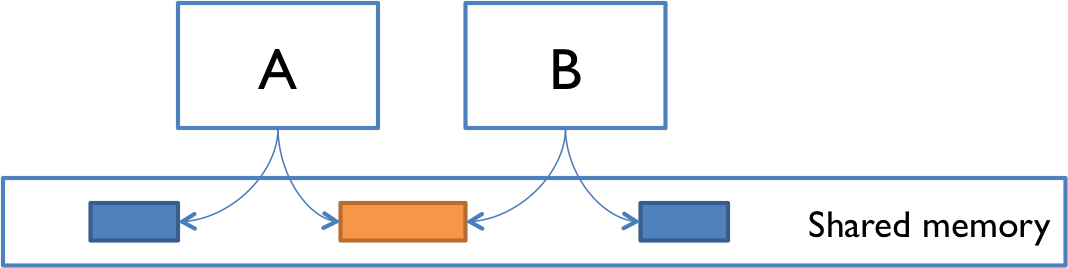
\includegraphics[scale=0.5]{./images/shared-memory.png}

\item Message passing

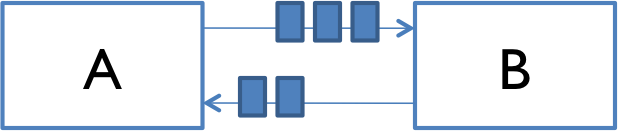
\includegraphics[scale=0.5]{./images/message-passing.png}

\end{enumerate}

Go uses the second approach, and to accomplish this it uses something called \textbf{channels}

\end{frame}

\begin{frame}[fragile]
\frametitle{Channels}

Channels are literally just, well, channels, between two goroutines -- things go in one end of the channel and out the other end.

The syntax for channels is actually clever:

\lstset{language=Go,
        basicstyle=\small\ttfamily,
        numbers=left,
		stepnumber=1,
		firstnumber=1,
		xleftmargin=2em,
		frame=single,
		framexleftmargin=2.5em,
		framexrightmargin=2em,
		numberfirstline=true,
		showstringspaces=false,
                keywordstyle=\color{blue}\ttfamily,
                stringstyle=\color{red}\ttfamily,
                commentstyle=\color{green}\ttfamily,
                morecomment=[l][\color{magenta}]{\#} 
} 
\begin{lstlisting}
// Create a channel that holds strings
messages := make(chan string)

// put 'ping' into the channel 
// (this typically happens in another thread)
messages <- "ping"

// read one message out of the channel
msg := <- messages
\end{lstlisting}

To be fair, you can use channels in C++ using Boost: \url{https://www.boost.org/doc/libs/1_65_0/libs/fiber/doc/html/fiber/synchronization/channels.html}

\vspace{0.5cm}

(Is there anything that \textit{isn't} in Boost?)
\end{frame}

\begin{frame}
\frametitle{Try not to aim for your foot}

In C++, to achieve \textit{safe}, concurrent code in applications that share data, you use:

\begin{itemize}
\item atomic types (see \href{https://en.cppreference.com/w/cpp/atomic/atomic}{std::atomic}) that have been guaranteed to be thread-safe
\item mutexes to synchronize access to some resource
\end{itemize}

Mess up on either of these and you're gonna have a bad time.

\end{frame}

\begin{frame}
\frametitle{Meanwhile}

Channels are inherently thread-safe in their implementation -- meaning data races aren't possible.

That being said, you do still have to worry about the traditional concurrency bugs.. deadlock, for example.

There are still some specific rules about how to use channels that you have to follow (e.g. not reading from an empty channel).

Also, if using a channel is overkill, you still \textit{can} use a traditional mutex like you would in C++.

\end{frame}

\begin{frame}
\frametitle{Odds and Ends}

We're going to switch gears a little bit to talk about a few more miscellaneous Go topics that didn't really fit in earlier. 

They are listed in decreasing order of importance:

\begin{itemize}
\item Generics
\item Interfaces
\item Slices
\end{itemize}

\end{frame}

\begin{frame}
\frametitle{"lol no generics"}

Right now, the single biggest criticism of Go is that it lacks generics. The simplest possible definition of "generics" is basically: writing code for a type but you don't know what that type is right now.

\vspace{0.5cm}

The problem this creates is that if you have a function \texttt{f} that works on an integer parameter, you have to re-write it a second time to work with strings.

\vspace{0.5cm}

Or do you?...


\hrulefill

\textit{This sounds really similar to templates, doesn't it? But.. templates (the way C++ does it) is actually an extension of the idea of 'generics', and the way they work under the hood is actually different than how generics work in a language for a Java for example. But that's a topic for a different day..}


\end{frame}

\begin{frame}[fragile]
\frametitle{Interfaces}

Well, actually, yeah you kind of do... BUT, there's one slight workaround called 'the empty interface'. 

First let's talk about what a regular interface looks like in Go:

\lstset{language=Go,
        basicstyle=\small\ttfamily,
        numbers=left,
		stepnumber=1,
		firstnumber=1,
		xleftmargin=2em,
		frame=single,
		framexleftmargin=2.5em,
		framexrightmargin=2em,
		numberfirstline=true,
		showstringspaces=false,
                keywordstyle=\color{blue}\ttfamily,
                stringstyle=\color{red}\ttfamily,
                commentstyle=\color{green}\ttfamily,
                morecomment=[l][\color{magenta}]{\#} 
}
\begin{lstlisting}
type polygon interface {
	area() float64
	perimeter() float64
}
\end{lstlisting}

We can now define our own structs, implement these methods, and then we can pass those objects to methods that take our interface as a parameter type:

\lstset{language=Go,
        basicstyle=\small\ttfamily,
        numbers=left,
		stepnumber=1,
		firstnumber=1,
		xleftmargin=2em,
		frame=single,
		framexleftmargin=2.5em,
		framexrightmargin=1em,
		numberfirstline=true,
		showstringspaces=false,
                keywordstyle=\color{blue}\ttfamily,
                stringstyle=\color{red}\ttfamily,
                commentstyle=\color{green}\ttfamily,
                morecomment=[l][\color{magenta}]{\#} 
}
\begin{lstlisting}
func printMeasurements(p polygon) {
    fmt.Println(p.area())
    fmt.Println(p.perimeter())
}
\end{lstlisting}

\end{frame}

\begin{frame}
\frametitle{Empty interface}

When you use an interface type as a function parameter, it tells the compiler: 'whatever type I pass into this function, must at least implement the methods of that interface'.

\vspace{0.5cm}

But the empty interface (denoted as \texttt{interface\{\}}), by definition, has no methods in it, so any possible type can be substituted for that interface. 

\vspace{0.5cm}

Consider a rollercoaster ride at an amusement park. The sign next to the ride says: \textit{you must be at least 48 inches tall to ride}. 

\vspace{0.5cm} 

If the sign instead said: \textit{you must be at least \underline{0} inches tall to ride} -- would there be anyone who \textbf{couldn't} go on that ride?

\end{frame}

\begin{frame}[fragile]

\frametitle{roll \textbf{C}all}

This concept should be familiar to C developers, who have been using \texttt{void*} similarly since the first World War.

\lstset{language=C,
        basicstyle=\small\ttfamily,
        numbers=left,
		stepnumber=1,
		firstnumber=1,
		xleftmargin=2em,
		frame=single,
		framexleftmargin=2.5em,
		framexrightmargin=1em,
		numberfirstline=true,
		showstringspaces=false,
                keywordstyle=\color{blue}\ttfamily,
                stringstyle=\color{red}\ttfamily,
                commentstyle=\color{green}\ttfamily,
                morecomment=[l][\color{magenta}]{\#} 
}
\begin{lstlisting}
int a = 1;
float b = 2.3;
void *p;
p = &a;
printf("Integer variable is = %d", *( (int*) p) );
p = &b;
printf("\nFloat variable is = %f", *( (float*) p) );
\end{lstlisting}

Mathematically, this concept is called a \textit{top type}*, and it exists in other common programming languages as well.
\end{frame}

\begin{frame}[fragile]
\frametitle{Slices}

Go, like any other sane language, has arrays. These are your pretty boring, fixed-size, same-type arrays, that you'd find in C.

\lstset{language=Go,
        basicstyle=\small\ttfamily,
        numbers=left,
		stepnumber=1,
		firstnumber=1,
		xleftmargin=2em,
		frame=single,
		framexleftmargin=2.5em,
		framexrightmargin=1em,
		numberfirstline=true,
		showstringspaces=false,
                keywordstyle=\color{blue}\ttfamily,
                stringstyle=\color{red}\ttfamily,
                commentstyle=\color{green}\ttfamily,
                morecomment=[l][\color{magenta}]{\#} 
}
\begin{lstlisting}
primes := [6]int{2, 3, 5, 7, 11, 13}
\end{lstlisting}

Slices, on the other hand, get used a bit more often. These are like dynamically-sized arrays, and are much easier to work with than slices.

You can create them through slicing an existing array or even just creating a slice directly:

\lstset{language=Go,
        basicstyle=\tiny\ttfamily,
        numbers=left,
		stepnumber=1,
		firstnumber=1,
		xleftmargin=2em,
		frame=single,
		framexleftmargin=2.5em,
		framexrightmargin=1em,
		numberfirstline=true,
		showstringspaces=false,
                keywordstyle=\color{blue}\ttfamily,
                stringstyle=\color{red}\ttfamily,
                commentstyle=\color{green}\ttfamily,
                morecomment=[l][\color{magenta}]{\#} 
}
\begin{lstlisting}
// One way to create a slice
primes := []int{2, 3, 5, 7, 11, 13, 17}

// Appending to a slice
primes = append(primes, 19)

// One way to initialize a slice
sliceOfAllZeros := make([]int, 5)

// Slice-ception
var s []int = primes[1:4]
\end{lstlisting}

\end{frame}

\begin{frame}
\frametitle{...}

So yeah. We've covered basically all the major topics in Go, and at this point you're pretty much ready to begin reading and writing basic Go code. 

The only things worth mentioning that I didn't get to talk about are:

\vspace{0.5cm}

\begin{itemize}
\item The \texttt{for} loop syntax
\item \texttt{select} statement
\item \texttt{defer} statement
\item The string system, e.g. strings, runes, bytes, etc.
\end{itemize}

\vspace{0.5cm}

For those interesting in learning more, I recommend you check out A Tour of Go: \url{https://tour.golang.org/}

\end{frame}

\end{document} 
